\documentclass[10pt,twocolumn]{article}

\usepackage{times,fullpage,hyperref,graphicx}
\renewcommand{\sectionautorefname}{\S}
\renewcommand{\subsectionautorefname}{\S}
\renewcommand{\subsubsectionautorefname}{\S}

\begin{document}

\title{\bf Probing for the Great Cannon}
\author{
	David M. Tagatac\\
	\texttt{dtagatac@cs.columbia.edu}
	\and
	Amit Levy\\
	\texttt{amit@amitlevy.com}
	\and
	Roxana Geambasu\\
	\texttt{roxana@cs.columbia.edu}
}
\date{}
\maketitle
\thispagestyle{empty}

%\begin{abstract}
%\input{abstr}
%\end{abstract}

\section{Introduction}
Marczak et al. presented evidence that the Great Firewall (GFW) is “on-path” and that the Great Cannon (GC) is “in-path”.~\cite{Marczak2015}
This means that the GFW cannot intercept packets, but only influences communications by inserting superfluous packets masqueraded as one of the endpoints.
The GC, on the other hand, can and has intercepted packets coming from Baidu’s servers and replaced them with their own packets – specifically to deliver a malicious JavaScript file as if it were from Baidu.
I have repeated a subset of their GFW experiments with similar results, and also shown that the GC is no longer behaving as it was during the DDoS attack on GitHub.
I have gone on to probe for other GC-like JavaScript file responses originating from some node in the path between Columbia and various domains on the Internet.

\section{The TTL Probe}
\subsection{Probing for the Great Firewall}
Before probing for the GC, I first verified that I was able to reproduce the results of Marczak et al.~\cite{Marczak2015} with respect to the GFW.
\subsubsection{Baseline}\label{gfwbaseline}
This experiment sent the message\\
\texttt{
	\-\ \ \ \ GET /?test HTTP/1.1\textbackslash{}r\textbackslash{}n\\
	\-\ \ \ \ Host: www.google.com\textbackslash{}r\textbackslash{}n\textbackslash{}r\textbackslash{}n\\
}
to IP address \texttt{123.125.65.120:80} via a STREAM socket 24 times, each time with a different TTL value, ranging from 1--24.
This is effectively requesting \texttt{www.google.com/?test} from a server (not Google) in Beijing with connectivity provided by China Unicom (Figure \ref{fig_gfwbaiduip}).
\begin{figure}
	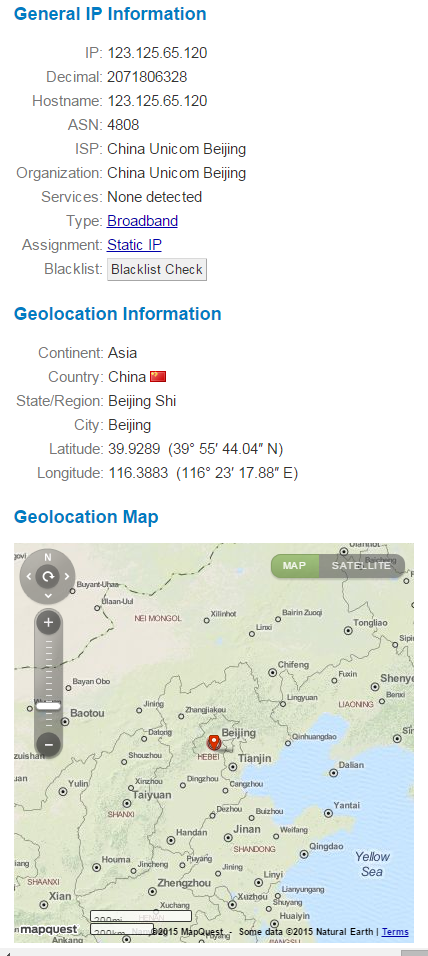
\includegraphics[width=\columnwidth]{figures/gfwbaiduip}
	\caption{
		Details on the destination IP address used in the experiments in \autoref{gfwbaseline} and \autoref{gfwlocation}.
		Note the location (Beijing) and the ISP (China Unicom).
	}
	\label{fig_gfwbaiduip}
\end{figure}

All of the requests prompted \texttt{Time-to-live exceeded} messages from intermediary nodes on the way to \texttt{123.125.65.120} until the request sent with TTL=24, which finally gets a \texttt{403} HTTP response (Figure \ref{fig_gfwtest}), as expected when requesting a google.com page from any server other than Google’s.
\begin{figure*}
	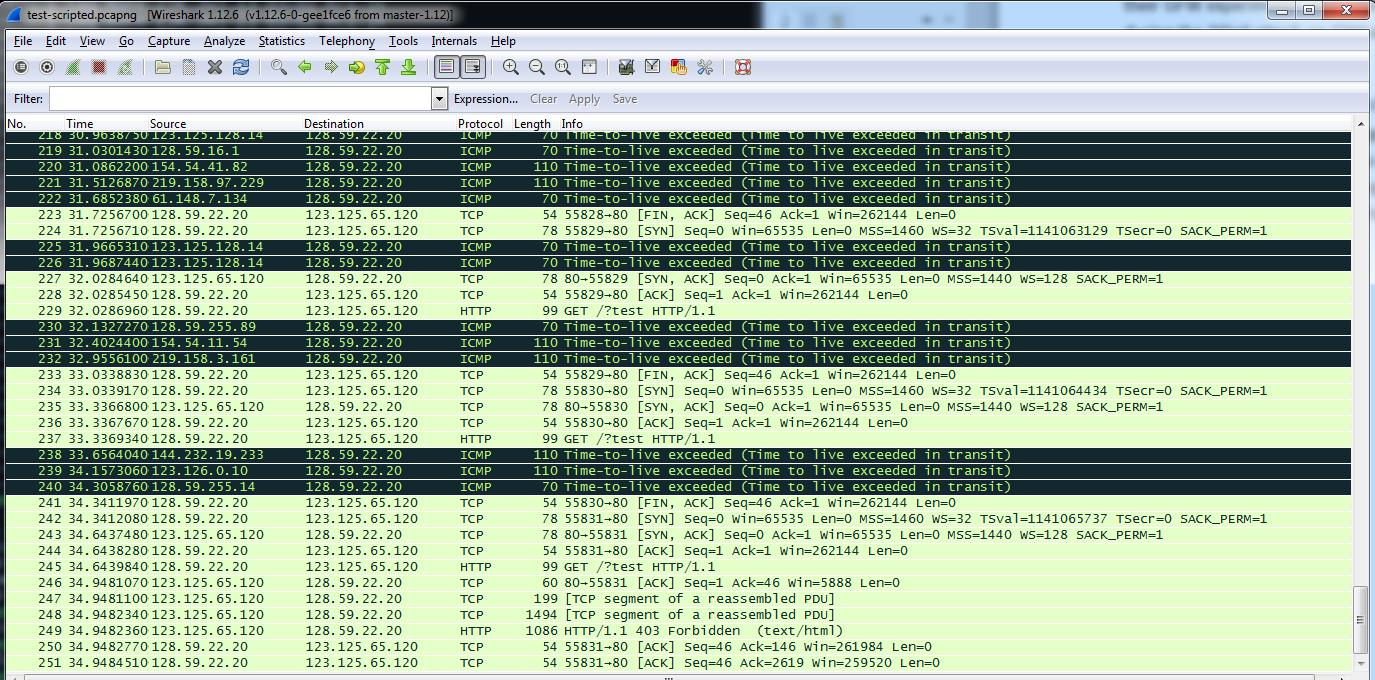
\includegraphics[width=\textwidth]{figures/gfwtest}
	\caption{
		No \texttt{[RST]} packets are sent when \texttt{www.google.com/?test} is requested from a Baidu server in Beijing.
		\texttt{Time-to-live exceeded} messages are received for small TTL values, until an HTTP response is received after sending the request with TTL=24 (packet 249), and the request reaches the Baidu server.
	}
	\label{fig_gfwtest}
\end{figure*}
The full packet capture can be found here: \url{https://github.com/tagatac/ttlprobe/blob/prelim/test-scripted.pcapng}.
The one spurious \texttt{[RST]} packet (packet 87) sent from my computer to \texttt{123.125.65.120} is a closing connection from a previous run of the same experiment.
You can see this from the port number used (55785), which is out of sequence with those from this experiment (55805--55831).
\subsubsection{GFW Location}\label{gfwlocation}
This experiment shows that the GFW is between 17 and 18 hops from my desktop along the path to \texttt{123.125.65.120}.
An identical experiment to Experiment 1 was performed, only substituting \texttt{falun} for \texttt{test} in the HTTP \texttt{GET} requests.
The results are the same as in \autoref{gfwbaseline} for TTL values 1--17.  For each TTL\textgreater=18, I received an \texttt{[RST]} packet and three \texttt{[RST, ACK]} packets apparently from \texttt{123.125.65.120} (but actually from GFW).
\texttt{[RST]} packets sent by the GFW to both endpoints (my desktop and the server and \texttt{123.125.65.120}) cause both to close the TCP connection.
The packet capture can be found here: \url{https://github.com/tagatac/ttlprobe/blob/prelim/falun-scripted.pcapng}.
The script used for both the experiments in \autoref{gfwbaseline} and \autoref{gfwlocation} can be found here: \url{https://github.com/tagatac/ttlprobe/blob/prelim/test.py}.
Figure \ref{fig_gfwfalun} shows the request with TTL=18 prompting the first \texttt{[RST]} packet from the GFW.
\begin{figure*}
	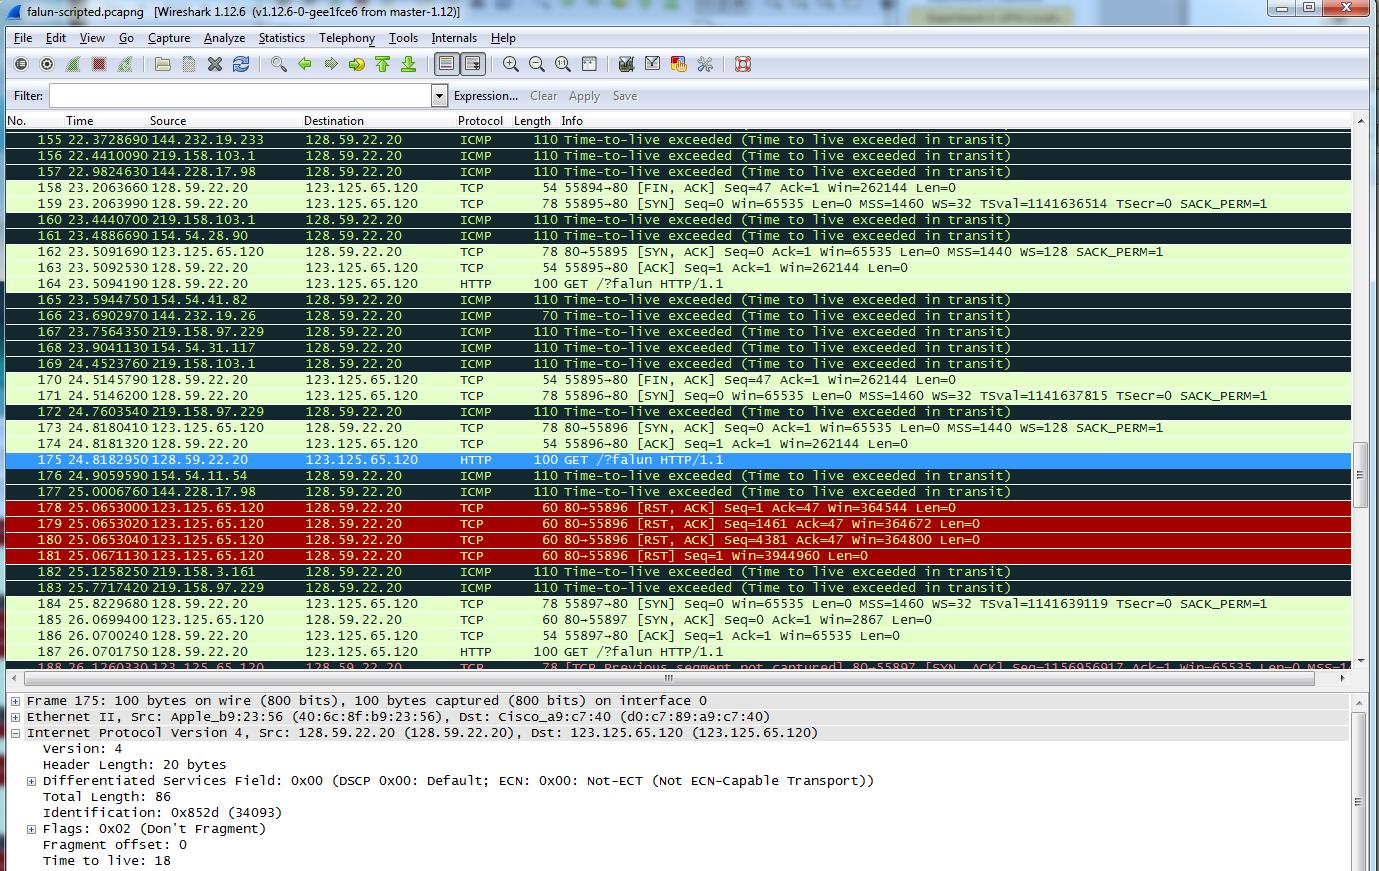
\includegraphics[width=\textwidth]{figures/gfwfalun}
	\caption{The GFW responds to the keywords \texttt{www.google.com/?falun} with several \texttt{[RST]} packets as soon as the request is sent 18 hops along the path to a Baidu server in Beijing.}
	\label{fig_gfwfalun}
\end{figure*}
\subsection{Probing for the Great Cannon}
\subsubsection{GitHub DDoS}
This experiment looked for GC packets as were observed during the DDoS on GitHub.
The observation specifically was a modified JavaScript file upon request for \texttt{hm.baidu.com/h.js}, an analytics tracking script similar to that used by Google Analytics.
The original can be found here: \url{https://github.com/tagatac/ttlprobe/blob/prelim/h.js}.
According to \mbox{NETRESEC}~\cite{Hjelmvik2015}, the modified file contains some obfuscated code that sends requests to GitHub in a 2-second loop.
Marczak et al. calculated that the substitution is made 1.75\% of the time, as long as your IP address is not ignored by the GC altogether, which happened to one of the machines they used for probing~\cite{Marczak2015}.
I ran a Python script (\url{https://github.com/tagatac/ttlprobe/blob/prelim/falunjs.py}) to download the analytics script for \texttt{7k7k.com} 1000 times.
MD5 hashes of every file match that of the unmodified JavaScript.

\section{Preparation for the GC Probe}
\input{prep}

\section{Results}
The probe was successfully run on the list of (referer, URI) pairs generated by the homepage-only crawler described in \autoref{homepages-crawler} in 4 hours and 22 minutes.
A histogram of the differences between the \texttt{scapy-python3}~\cite{Dobelis2015} traceroute result for the serving domain and the minimum TTL value required to obtain each file is shown in Figure~\ref{fig_histhomepages}.
All files which were successfully downloaded were received for TTL values within 2 hops of the estimated distance to their respective servers.
Only 30 files were received for TTL values less than the estimated distance to their respective servers.
\begin{figure}
	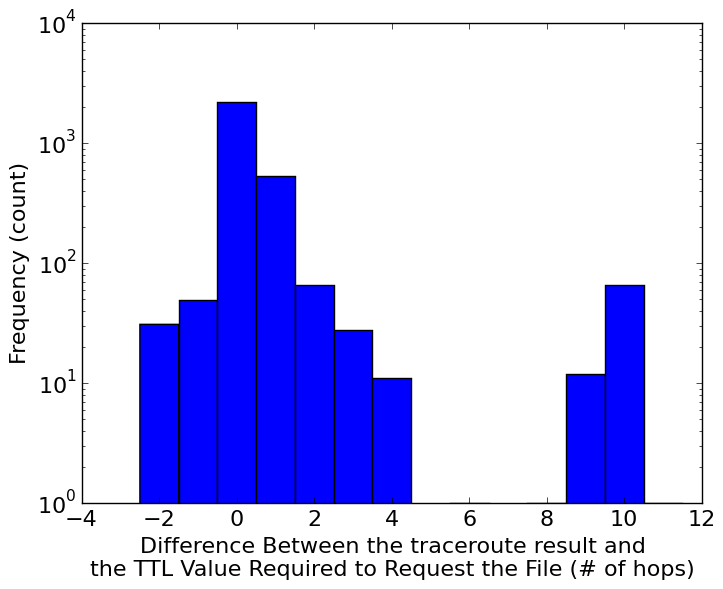
\includegraphics[width=\columnwidth]{figures/histhomepages}
	\caption{
		A histogram showing how often a file request succeeded with a TTL value less than the number of hops to the server (as estimated by the \texttt{scapy-python3}~\cite{Dobelis2015} traceroute), when downloading files from URIs scraped by the homepage-only crawler.
		A zero value on the x-axis represents files which were not received until the TTL value of the request was set to the result of the traceroute.
		Larger values on the x-axis represent files which were received when the TTL value of the request was less than the result of the traceroute.
		Negative values represent files which were not received until the TTL value of the request was set to be greater than the result of the traceroute.
		Files which were not received even when the request was sent with a TTL value 3 greater than the traceroute result are not shown.
	}
	\label{fig_histhomepages}
\end{figure}

Another probe is in progress on the partial list of 0.9 million (referer, URI) pairs generated by the full-site crawler described in \autoref{full-crawler}.
Through 20 hours, 15,662 files have been probed.
A histogram of the differences between the traceroute result for the serving domain and the minimum TTL value required to obtain each file is shown in Figure~\ref{fig_histmemfail}.
\begin{figure}
	\includegraphics[width=\columnwidth]{figures/histmemfail}
	\caption{
		A histogram showing how often a file request succeeded with a TTL value less than the number of hops to the server (as estimated by the \texttt{scapy-python3} traceroute), when downloading files from URIs scraped by the full-site crawler prior to failure in DFO mode.
	}
	\label{fig_histmemfail}
\end{figure}

\section{Other Applications of TTL Probing}
\subsection{Assumptions}
This probe makes a number of assumptions.
First, it assumes that the injection rate of the GC or other injector (assuming there is one and it is active) is high enough that testing each TTL value in the binary search for the minimum TTL value required yields a significant chance that an injection will be seen.
Injection rates seen by Marczak et al. were about 1.75\%~\cite{Marczak2015}.
Second, it assumes that one or more of the files for which the crawlers scraped URIs is being targeted by the GC or other injector.
In the case of the GitHub DDoS, only a single file was seen to be targeted.
Finally, it assumes that the IP address from which the probe is run is not being filtered.
Marczak et al. observed that no injections were made in response to requests originating from one of four test IP addresses.
\subsection{Next Steps}
Several technical improvements can be made to the probing process:
\begin{itemize}\addtolength{\itemsep}{-.35\baselineskip}
	\item As the probe for a given domain can often run for a long time, it may be advantageous to perform multiple \texttt{traceroute}s throughout the course of a probe to increase temporal proximity in the distance estimates.
		Additionally, a better estimate for the distance of a domain's servers may be possible, perhaps using the TTL value required to download other files from that domain.
	\item DNS lookup failures can be handled more gracefully.
	\item The full-site crawler can be optimized for broad crawls.
		Several suggestions are offered on the Scrapy website: \url{http://doc.scrapy.org/en/latest/topics/broad-crawls.html}
	\item The crawlers can also do a better job at scraping JS URIs.
		At present, all relative URIs and URIs containing single quotes are ignored.
\end{itemize}

An obvious extension to these one-off probes would be a persistent probe running in a slow loop so as to avoid detection and wasting network resources.
By triggering alerts when suspicious files are found, this persistent probe would be in a good position to detect future GC activity.

\section{Conclusion}
Basic GFW results were repeated.
A preliminary probe for GC-like activity was conducted.
A test in a controlled environment where I initiate file injections myself confirms that the probe works as intended.
Some more analysis on the data recorded after probing the partial file list from the DFO full-site crawl is needed.
It is still not clear how to use this method to probe for anything other than GC-like activity, but a persistent scan and/or testing other malicious-injection detection tools could be interesting.

{\footnotesize \bibliographystyle{acm}
\bibliography{refs}}

\end{document}
